\documentclass[paper=a4, fontsize=11pt]{scrartcl}
\usepackage[T1]{fontenc}
\usepackage{fourier}

\usepackage[english]{babel}															% English language/hyphenation
\usepackage[protrusion=true,expansion=true]{microtype}	
\usepackage{amsmath,amsfonts,amsthm} % Math packages
\usepackage[pdftex]{graphicx}	
\usepackage{url}
\usepackage{hyperref}

%%% Custom sectioning
\usepackage{sectsty}
\usepackage{graphicx}

\graphicspath{ {images/} }
\allsectionsfont{\centering \normalfont\scshape}


%%% Custom headers/footers (fancyhdr package)
\usepackage{fancyhdr}
\pagestyle{fancyplain}
\fancyhead{}											% No page header
\fancyfoot[L]{}											% Empty
\fancyfoot[C]{}											% Empty
\fancyfoot[R]{\thepage}									% Pagenumbering
\renewcommand{\headrulewidth}{0pt}			% Remove header underlines
\renewcommand{\footrulewidth}{0pt}				% Remove footer underlines
\setlength{\headheight}{13.6pt}


%%% Equation and float numbering
\numberwithin{equation}{section}		% Equationnumbering: section.eq#
\numberwithin{figure}{section}			% Figurenumbering: section.fig#
\numberwithin{table}{section}				% Tablenumbering: section.tab#


%%% Maketitle metadata
\newcommand{\horrule}[1]{\rule{\linewidth}{#1}} 	% Horizontal rule

\title{
		\usefont{OT1}{bch}{b}{n}
		\normalfont \normalsize \textsc{COMP3211 Software Engineering} \\ [25pt]
		\horrule{0.5pt} \\[0.4cm]
		\huge Software requirements and design specifications
		\horrule{2pt} \\[0.5cm]
}
\author{
		\normalfont 								
        FU Kuo-hao \\
        14112466D
        \and
        OUYANG Xiating \\
        14111773D
        \and
        ZHOU Yi \\
        14109328D
}
\date{\today}


%%% Begin document
\begin{document}
\begin{titlepage}
\maketitle

\end{titlepage}

\begin{titlepage}
\tableofcontents
\end{titlepage}


\section{Software Requirement Specification}

\subsection{Introduction}
This document will include all requirements and functionalities of Edo, a course management system for the Edward University of Smartness (EUS). This document will summarize the specifications and requirements obtained from Edward, who is the president of EUS, and our proposed design of Edo.

\subsubsection{Definitions}
The following abbreviations are used throughout this document.
\begin{enumerate}
	\item Course content: the slides, notes or other course related files
	\item Assessment: assignment and quiz
	\item User: students and professors
	\item File: any document uploaded to Edo, including course slides, note, assignment instruction etc.
\end{enumerate}

\subsubsection{Goals and objectives}
This project aims at developing an online course management system (Edo) for Edward University of Smartness (EUS). It offers EUS a lightweight platform which is supposed to help teachers distribute their course content and assess the performances of their students, while students can have easy access to course resources and finish assignments or quizzes on this platform.

\subsubsection{Statement of scope}
\begin{enumerate}
	\item Description
	\par Edo is a course management system for both professors and students where professors can upload assignments and set up quizzes and students can upload their assignment answers and complete quizzes. After the quizzes and assignments are assessed, the grades can be given to students by professors and students may login their accounts to view their grades.
	\item Major inputs
	\par Major inputs include course resources, such as notes, assignment files and quiz questions from teachers and assessment submissions from students.
	\item Processing Functionality
	\par Edo should be able to store the uploaded file and course assessment information and return the corresponding results, such as the desired course content and attempted grades correctly and efficiently.
	\item Outputs
	\par Course contents are returned in the form of a web link displayed on the screen. The grades for each assignment and quiz are also available. If a user intend to download a file from Edo, the correct file should be returned.
	\item Functionality priority
	\begin{itemize}
		\item Essential
		\begin{itemize}
			\item Correctness, all files should be returned correctly and no wrong file or content should be returned
			\item Basic security: We guarantee the integrity of the users and confidentiality of data processed.
			\item Availability, the system should be available 24/7, as the students and professors should be able to access Edo anytime for uploading and viewing files.
		\end{itemize}
		\item Desirable
		\begin{itemize}
			\item More security issues: the system should be immune from DDoS attack; the system should be able to detect malicious accesses.
			The system allows users to upload files from third-party storage systems like Google Drive, Dropbox, Onedrive, etc.
			\item Customizability: The users may choose to customize their personal homepage when displaying the course information.
		\end{itemize}
		\item Future
		\begin{itemize}
			\item Speed: the files should be uploaded and returned at at least 500Kb/s since otherwise a student might miss the deadline due to the low transmission speed.
		\end{itemize}
	\end{itemize}	
\end{enumerate}

\subsubsection{Software context}
Edward is the president of a newly founded university, Edward University of Smartness. EUS has recruited professors and admitted undergraduate students, and it needs a learning platform for professors to post assignments and quizzes, and for students to upload assignments and complete quizzes. Therefore, Edward would like to hire our programming team to develop a course management system Edo, for EUS.
\subsubsection{Major constraints}
The development of Edo is mostly limited by the time of delivery since the EUS will start its first semester in 2017 Fall and the system is in urgent need. Therefore this project will only deliver the core functionality of Edo. After delivery, Edo will be further refined in future endeavors.

\subsection{Usage scenario}

\subsubsection{User profiles}
\begin{itemize}
	\item The students of EUS: This user will have the access to his/her registered courses and view all the related course contents. They can also submit the assignment answers and answer quiz questions posted on Edo.
	\item The professors (and Teaching assistants) of EUS: This user will have access to create the course information in Edo and upload corresponding course materials, including course note, course assignment and quizzes on Edo for students' reference.
\end{itemize}


\subsubsection{Use-cases}
\begin{itemize}
	\item Use-Case Descriptions \footnote{The later usecases are presumed to be performed while staying logged in.}
	\par Student/Professor logs in
	\begin{enumerate}
		\item The user enters his/her username and password, and clicks the enter button.
		\item The user logs in Edo and enter his/her personal homepage.
	\end{enumerate}
	\par Student views course
	\begin{enumerate}
		\item The student clicks a course displayed on the personal homepage.
		\item The course notes, assignments and quizzes are shown.
	\end{enumerate}
	\par Student views course content
	\begin{enumerate}
		\item The student clicks one course note, and the course note is downloaded.
	\end{enumerate}
	\par Student answers assignment
	\begin{enumerate}
		\item The student clicks one assignment, and the assignment introduction and guide is displayed.
		\item The student upload his answer to the assignment to Edo.
		\item The student clicks finish button to finish, and returns to course information page.
	\end{enumerate}
	\par Student answers quiz
	\begin{enumerate}
		\item The student clicks one course quiz, and the quiz questions are displayed.
		\item The student chooses one of the four choices for each quiz question by ticking the box ahead of each choice, and clicks submit button.
		\item The student clicks the completed assignment and quiz, the grades, if available, will be shown to them. 
	\end{enumerate}
	\par Professor logs off
	\begin{enumerate}
		\item The student clicks the logoff button
		\item The student is logged off.
	\end{enumerate}
	\par Professor views courses
	\begin{enumerate}
		\item The professor enters his/her username and password, and clicks the enter button.
		\item The professor enters the personal homepage, and clicks on a course he teaches.
	\end{enumerate}
	\par Professor creates assignment
	\begin{enumerate}
		\item The professor clicks the create content button, and chooses one file from his/her PC for upload.
		\item The professor clicks the create assignment button, and enters the assignment information and chooses a file for that assignment.
		\item The professor clicks the submit button, and the assignment is created.
		\item The professor clicks the assignment submission button to view all assignment submissions, and give grades to those submissions by entering the grades in the grade bar.
	\end{enumerate}
	\par Professor creates quiz
	\begin{enumerate}
		\item The professor clicks create quiz.
		\item The professor enters the name of the quiz.
		\item The professor sets up one MC question.
		\item The professor enters the description of the MC question.
		\item Then, the teacher enters the four options for the MC question.
		\item The professor sets up the correct answer.
		\item The professor continues 9-12, until all questions are set.
		\item The professor clicks ``finish" button, and the quiz is created and henceforth posted.
	\end{enumerate}
	\par Professor logs off
	\begin{enumerate}
		\item The professor clicks the logoff button.
		\item The professor is logged off the system.
	\end{enumerate}
	
	\item Use-Case Diagram
	\begin{figure}[!ht]
		\begin{center}
			%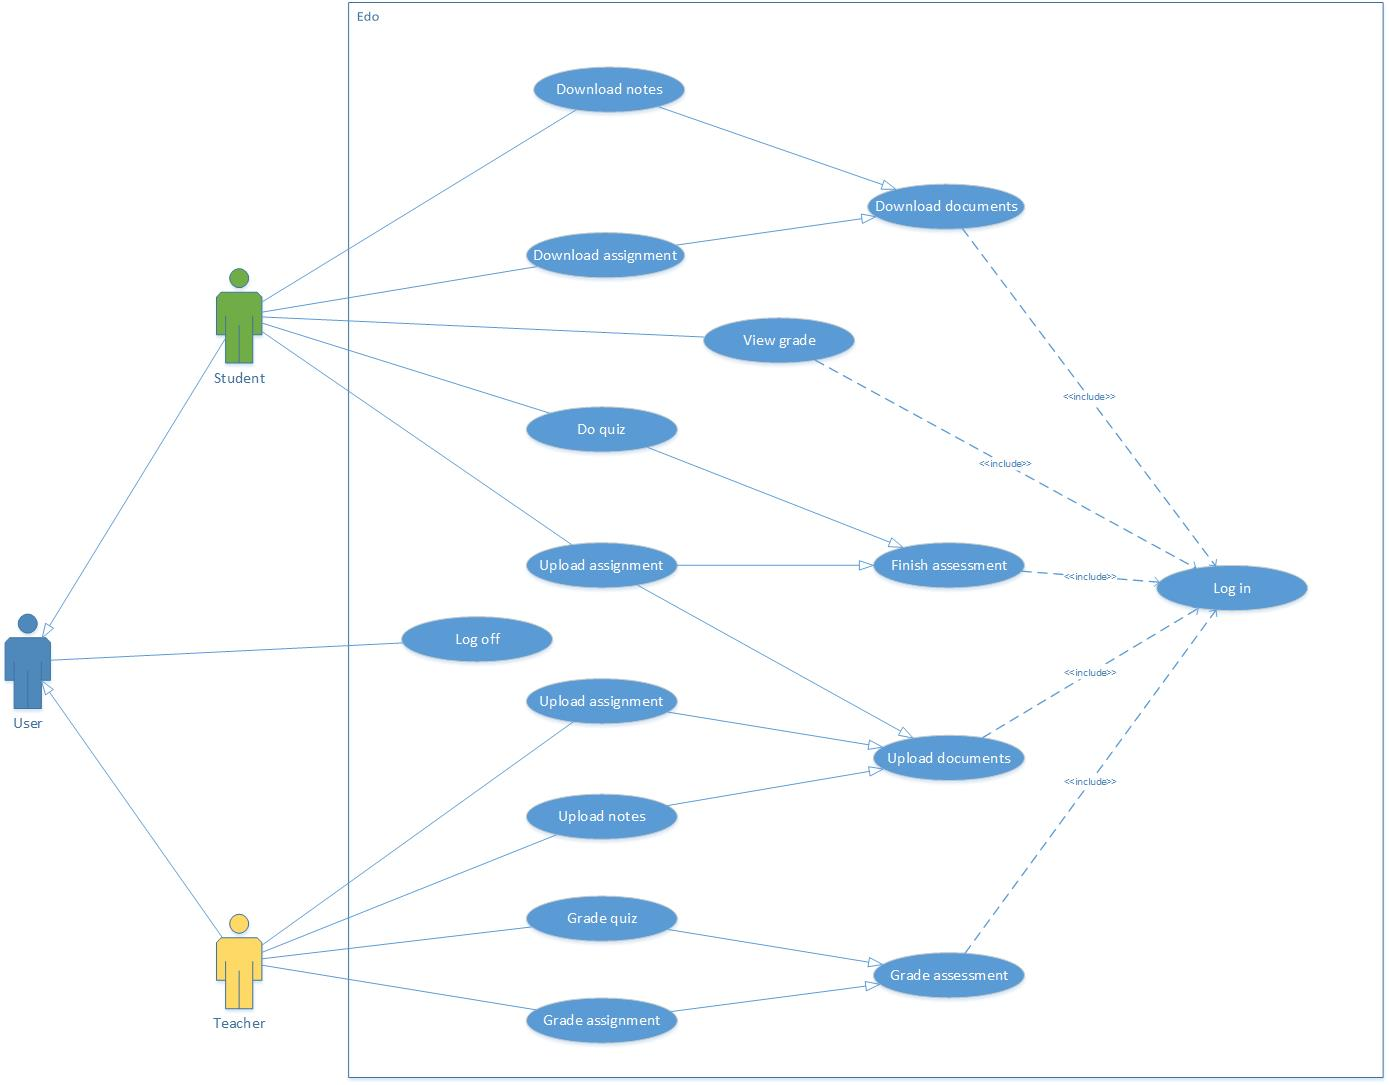
\includegraphics[width=\textwidth,height=\textheight,keepaspectratio]{usecase}
		\end{center}
		\caption{Use case diagram}
	\end{figure}
	
\end{itemize}



\subsection{Data Model and Description}

\subsubsection{Data objects}
The users will have username and password for authentication. After login, their first name and last name will be displayed on the homepage. For professors, they additionally have titles and institutions, which are useful in future refinements.

A course has course contents, assignments and quizzes. Contents will be simple .doc or .pdf files, and an assignment will contain a description and a supplementary file, if deemed necessary. Quizzes will have multiple MC questions with four choices each. Each quiz question will have one correct answer. Students will submit their quiz or assignment submission, which may contain a supplementary file if deemed necessary. Grade is either a floating point value or A, B, C, D, F (and their subgrades), and is associated with assignment and quiz submissions.

\subsubsection{Relationships}
One student may take multiple courses, and one professors may teach multiple courses. For each course, it has multiple course contents, courses assignments and course quizzes. Each quiz has multiple questions and each question will have four choices. Each assessment will have multiple submissions from students, and each student submission will have only one grade. 

\subsubsection{Complete data model}
\begin{figure}[!ht]
	\begin{center}
		%\includegraphics[width=\textwidth,height=\textheight,keepaspectratio]{datamodel}
	\end{center}
	\caption{Data Model of Edo}
\end{figure}


\subsection{Behavioral Model and Description}

\subsubsection{Description for software behavior}

\begin{itemize}
	\item Events
	\begin{itemize}
		\item Student/professor login: this event will guide the students or professors to their homepages.
		\item Click on course: click on the course, content, assignment, quiz and grade.
		\item Click on course content
		\item Click on course assignment
		\item Click on course quiz
		\item Click on assignment/quiz grade
		\item Submit assignment
		\item Submit quiz
		\item Create assignment
		\item Create quiz
		\item Create content
	\end{itemize}
	\item States
	\begin{itemize}
		\item Logged off state
		\item Student logged in state
		\item Professor logged in state
		\item View course content state: course content including notes, assignments and quizzes are displayed.
		\item View notes, assignment, quiz states: the corresponding content is displayed.
		\item Do assignment, quiz states: the answers are stored by the system and ready for upload.
		\item Upload content, assignment, quiz state: the content, assignment and quiz is being prepared and completed by professors and is ready for upload.
		\item Grade: the professors are giving grades to the submitted assignment. \footnote{Quizzes are auto graded since each quiz question is set with a correct answer.}
		\item View grade: the students may view their attempted grades of assignments and quizzes.
	\end{itemize}
\end{itemize}

\subsubsection{State-chart Diagram}
\begin{figure}[!ht]
	\begin{center}
		%\includegraphics[width=\textwidth,height=\textheight,keepaspectratio]{statechart}
	\end{center}
	\caption{State Chart Diagram of Edo}
\end{figure}


\subsection{Restrictions, Limitations, and Constraints}
The size of files uploaded should not exceed the maximum size (5MB so far), otherwise the server will not be able to store all of the files.

The students are expected to complete the course and they cannot drop the registered course half way.

The course list will be retrieved from the course registration system. Edo only serves as a platform to share teaching materials and post assessments.

Edo is highly dependent on network performance, and thus the response time is not well guaranteed.


\section{Software Design Specification}


\subsection{Architectural and component-level design}
This section will focus on the design of Edo in terms of its components, and it is shown through its class diagram.

\subsubsection{Class Diagram}

\begin{figure}[!ht]
	\begin{center}
		%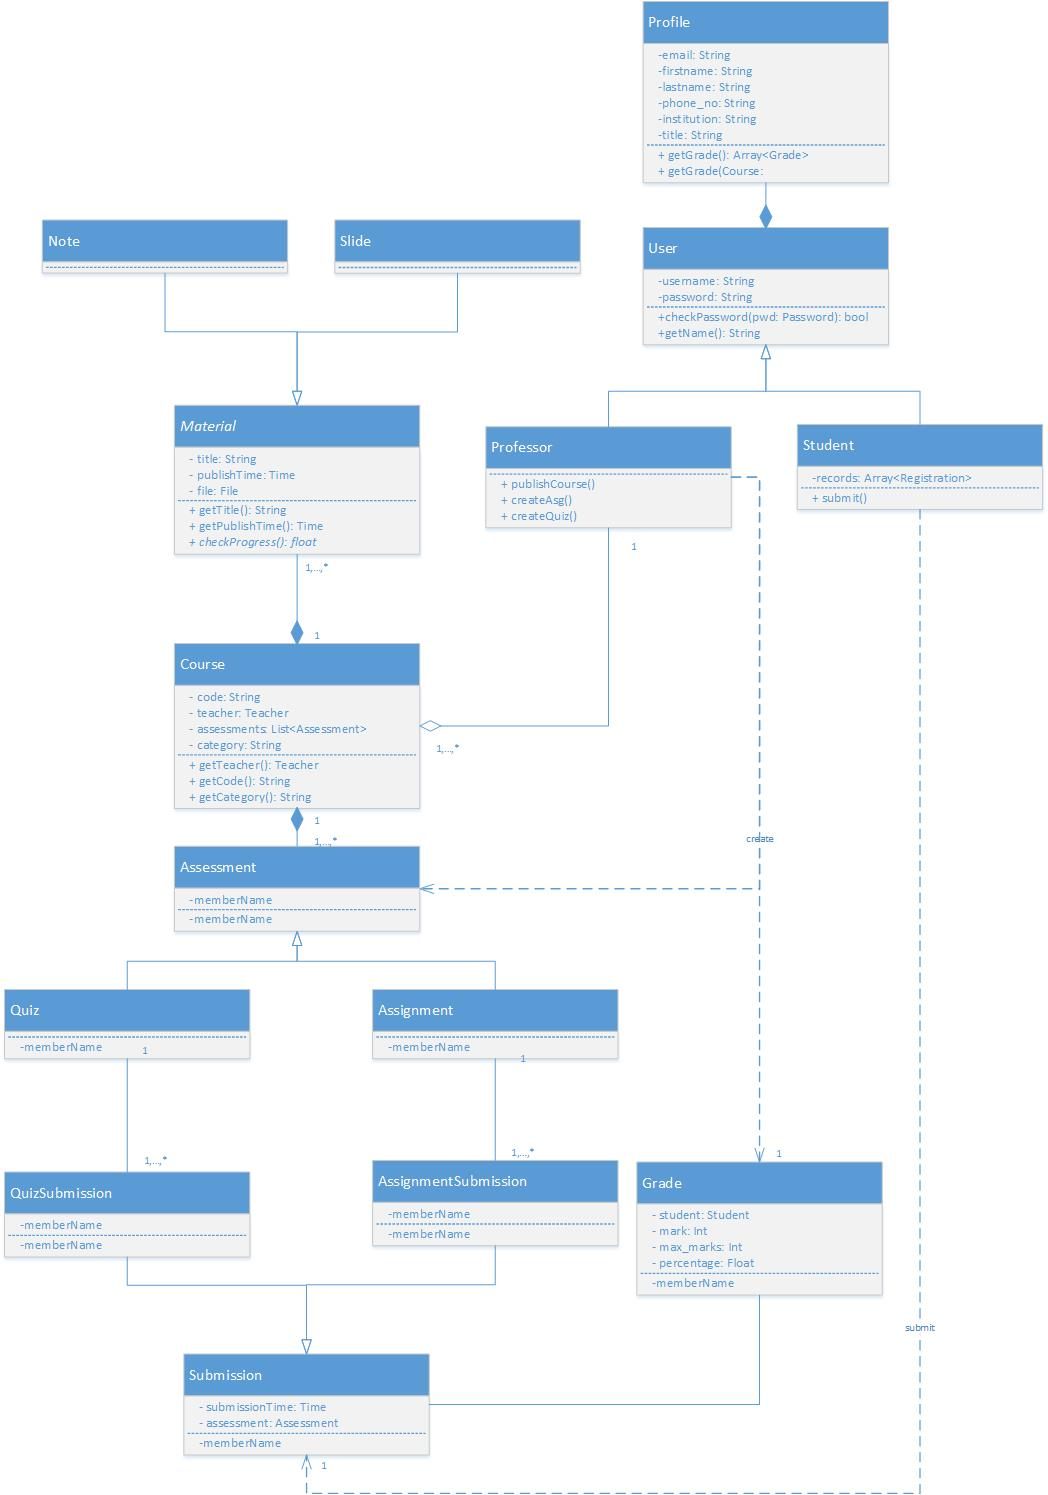
\includegraphics[width=\textwidth,height=\textheight,keepaspectratio]{class}
	\end{center}
	\caption{Class Diagram of Edo}
\end{figure}


\subsection{Description for Components}

The following components together perform the essential functionalities of Edo. All components rely on and are triggered by the user event handler, which is a widely used web component. Therefore web components are omitted for the component interface part.

%%%%%%%%%%%%%%%%%%%%%%%%%%%%%%%%%%%%%%%%%%%%%%%%%%%%%%%%%%%%%%%%%%%%%%%%%%%%%%%%%%%%%%%%%%%%%%%%%
%Refer to this page http://www.codingthearchitecture.com/2015/03/31/components\_vs\_classes.html%
%%%%%%%%%%%%%%%%%%%%%%%%%%%%%%%%%%%%%%%%%%%%%%%%%%%%%%%%%%%%%%%%%%%%%%%%%%%%%%%%%%%%%%%%%%%%%%%%%
\subsubsection{Login Component}
\begin{enumerate}
	\item Processing narrative for component
	\par This component will be responsible for user login. The user enters the username and password, and if they match, the user is thereafter logged in.
	\item Components interface description
	\par This component will have an interface with the account system of EUS to validate the username and password since the student account information is only stored in the account system.
	\item Components processing detail
	\begin{itemize}
		\item Restrictions/limitations for component
		\par This component does not hold the specific login information as duplication of student accounts may bring security hazards.
		\item Performance issues for component 
		\par This component should be correctly implemented and run securely since it involves privacy issue. Therefore the performance overhead might be large since it involves security and network transmission, a conflict of interest between stakeholders students and security managers.
		\item Design constraints for component 
		\par Login is largely dependent on the transmission between Edo and the account system, and thus the responsiveness may not be guaranteed. The username and password will be limited to a maximum of 32 characters.
		\item Processing detail for each operation of component 
		\par First, the system will call a function from the account information system of EUS for login operation. Then, a login form is displayed on the screen, and the user will enter his/her username and password into the form. The input is authenticated by the account information system. All of the authentication details are encapsulated in the account information system. After login, a token will be returned from the account information system. If the token is valid, the user will be logged in.
	\end{itemize}
\end{enumerate}

\subsubsection{Course retrieval}
\begin{enumerate}
	\item Processing narrative for component
	\par This component will retrieve the course registration information from the registration system as the semester begins and initialize the database of assignments, notes and quizzes for each course.
	\item Components interface description
	\par This component will retrieve the courses taken/taught by the users and use that information to initialize the database.
	\item Components processing detail
	\begin{itemize}
		\item Restrictions/limitations for component
		\par The retrieval process is run right after the registration period finishes. Therefore the students are strictly not allowed to drop any course from the course registration system after the course registration period. 
		\item Performance issues for component 
		\par This system also greatly relies on the network performance, and the data to be transmitted is large in size. Therefore, it may take several minutes to finish the retrieval process. 
		\item Processing detail for each operation of component 
		\par Edo will query the course registration system for course registration information and stores related initialize its own database through the data obtained.
	\end{itemize}
\end{enumerate}

\subsubsection{Resource Uploading}
\begin{enumerate}
	\item Processing narrative for component
	\par This component will handle the uploading request made by professors and students.
	\item Components interface description
	\par This component will send the uploaded file to the resource management system for storing purpose.
	\item Components processing detail
	\begin{itemize}
		\item Restrictions/limitations for component
		\par This component is sensitive to the input file size, and the size of each file should be limited to maximum 5 MB.
		\item Performance issues for component 
		\par The performance might decline as the number of files to be submitted grows.
		\item Processing detail for each operation of component 
		\par The user chooses one file to be uploaded, and clicks the submit button. This component will forward the file to the resource management component, and redirect the user back to the course information page.
	\end{itemize}
\end{enumerate}


\subsubsection{Resource Management}
\begin{enumerate}
	\item Processing narrative for component
	\par This component stores all the files and information that a professor uploads and a student submits, and maintains the link between the students and their registered courses.
	\item Components interface description
	\par This component will have an interface with the user interaction component to exchange data with the users.
	\item Components processing detail
	\begin{itemize}
		\item Restrictions/limitations for component
		\par This component is sensitive to the input file size, and the size of each file should be limited to maximum 5 MB.
		\item Performance issues for component 
		\par The performance might decline as the number of files grows.
		\item Processing detail for each operation of component 
		\par When the user uploads a file to assignment or content, this component will record the label of that origin and associate the uploaded file with the fingerprint of that origin. Later when the document is requested by the user, this component will retrieve the file using the origin and return it to the user.
	\end{itemize}
\end{enumerate}


\subsection{Interface design}	


\subsubsection{External machine interface}
Edo will be an online platform and thus the users are required to use the browser and enter the URL or Edo to access this system. The physical machine could be either PC or tablets.

\subsubsection{External system interface}
Edo will be exchanging data with the student account system and the web system that carries out the data transmission. 

\subsubsection{Description of the user interface}
This prototype of the Edo user interface is shown as below.
\begin{figure}[!ht]
	\begin{center}
		%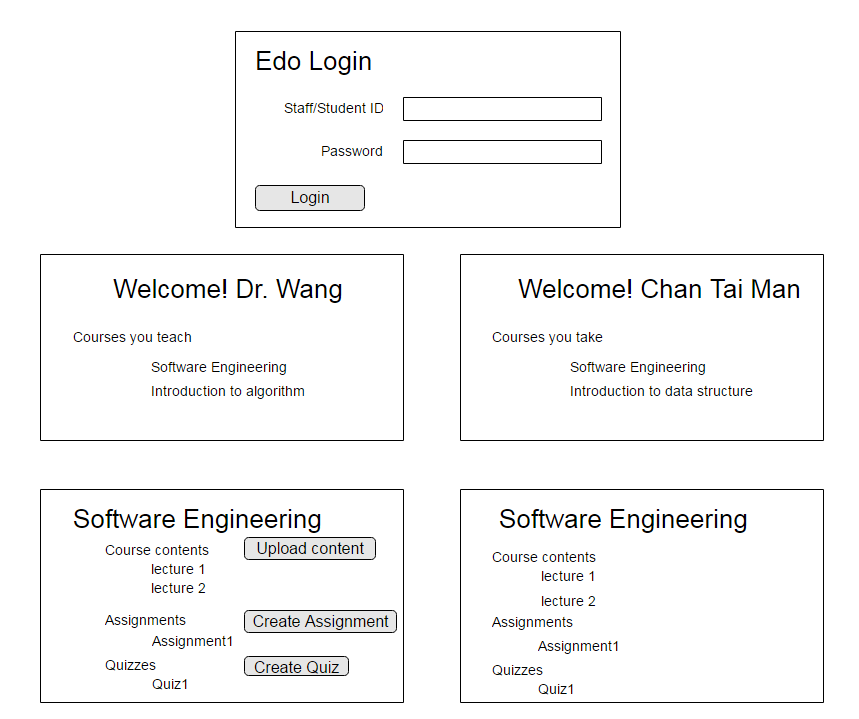
\includegraphics[width=\textwidth,height=\textheight,keepaspectratio]{interface}
	\end{center}
	\caption{User interface}
\end{figure}




\subsubsection{Interface design rules}
The interface should have high clarity to facilitate the use of Edo. In each page, only the navigation bar and the corresponding content shall be visible. E.g. in course information page, only the course notes, course assignment and couse quiz will be displayed, but in course note, course assignment and quiz will not be shown.

\subsubsection{Interface Components available}
Edo will be put online and thus all the web based components, such as bootstrap, javascript and angular js are all available for development. 


\subsection{Restrictions, limitations, and constraints}
The design of Edo is very compact that the interface may not look quite fancy. It only supports a few core functionalities so far, and more can be added in the future evolution process.

This physical design does not include the network layer components, and is dependent on the network performance.
\subsection{Testing Issues}

\subsubsection{Classes of tests}
\begin{enumerate}
	\item Login: Entering the username and password wrongly.
	\item Creation: create an assignment or quiz by entering the name and description.
	\item View: view an assignment by clicking on the assignment title.
	\item Download file: Edo should return the correct file to be downloaded to the students.
	\item Submission of assignment and quiz: submit a file or quiz response to the system.
	\item Invalid upload file: The file to be uploaded to Edo is not supported.
\end{enumerate}
\subsubsection{Expected software response}
\begin{enumerate}
	\item Login: An error message shall pop up and the user to be directed to login again.
	\item Creation: the assignment, content and quiz should be created and viewable in both professors' and students' homepages.
	\item View: The students can see the courses and the related materials in their homepages.
	\item Download file: The correct file that the student desires should be downloaded to the client side.
	\item Submission of assignment and quiz: the file is submitted to Edo and professors can see the submission from Edo.
	\item Invalid upload file: An error message shall pop up and redirect the user to upload again.
\end{enumerate}

\subsubsection{Performance bounds}
Since most of the functionalities are dependent on network performance, quick response is not guaranteed. Efforts will be spent on ensuring the turnaround time of each functionality is bounded by 2 seconds. 

\subsubsection{Identification of critical components}
The critical components are the login component and resource management component. Login component should ensure the overall security of the system, and the resource management component is responsible for efficient material retrieval and delivery process. The resource management component shall index the uploaded materials properly to achieve high efficiency.
\end{document}


